% biography section
% 
% If you have an EPS/PDF photo (graphicx package needed) extra braces are
% needed around the contents of the optional argument to biography to prevent
% the LaTeX parser from getting confused when it sees the complicated
% \includegraphics command within an optional argument. (You could create
% your own custom macro containing the \includegraphics command to make things
% simpler here.)
% or if you just want to reserve a space for a photo:

%\begin{IEEEbiography}{Yu-Jiu Wang  (S'04 - M'09)}
%\begin{IEEEbiography}[{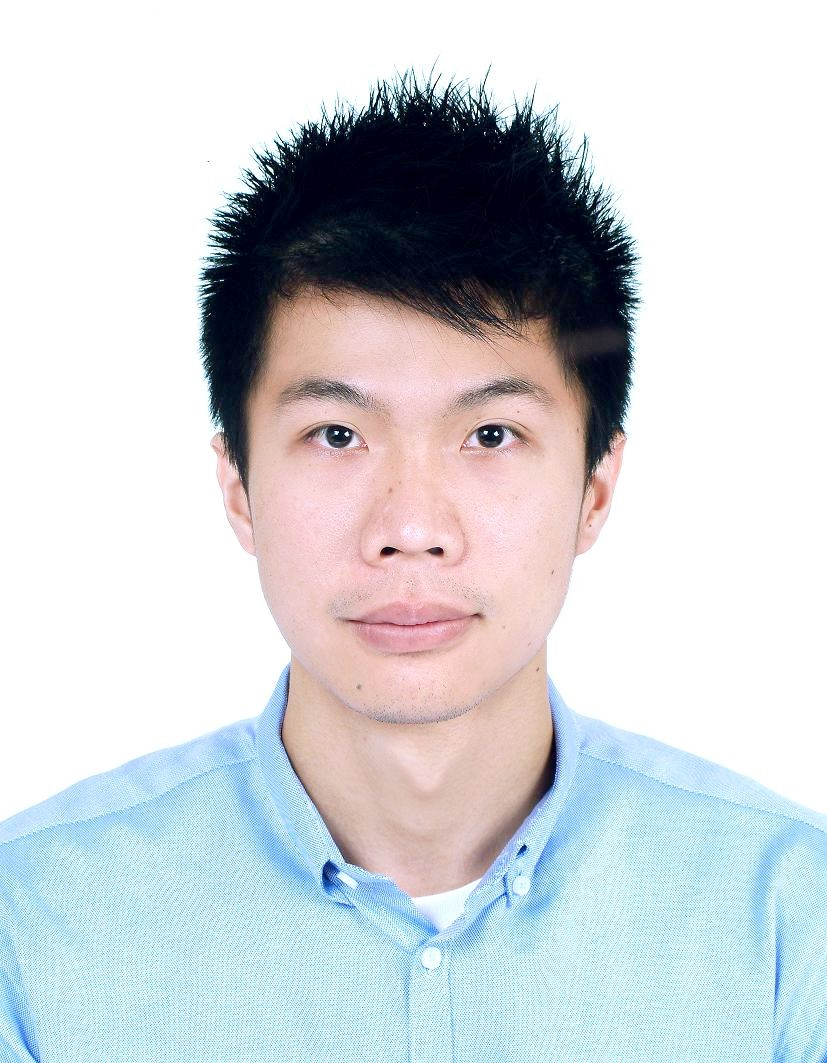
\includegraphics[width=1in,height=1.25in,clip,keepaspectratio]{\imag\yujiu.jpg}}]{Yu-Jiu Wang  (S'04 - M'09)}

\begin{IEEEbiography}[{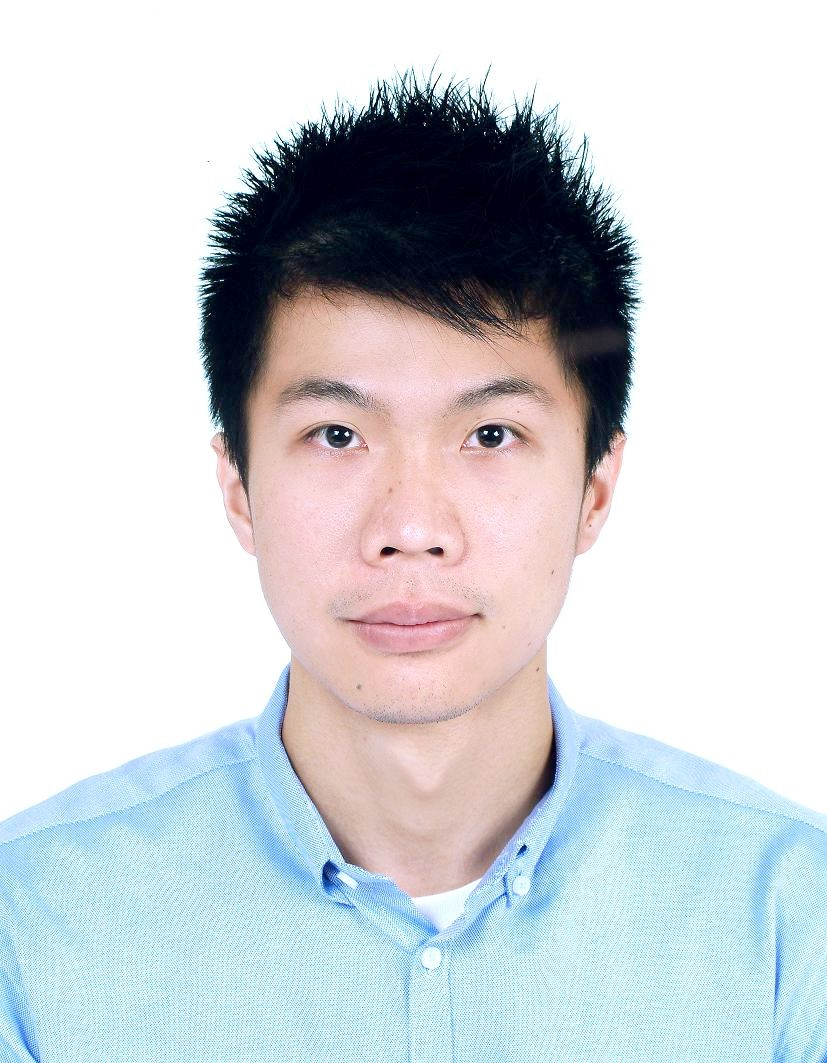
\includegraphics[width=1in,clip,keepaspectratio]{yujiu}}]{Yu-Jiu Wang  (S'04 - M'09)}


received the B.S. degree in electrical engineering from National Taiwan University (NTU), Taipei, Taiwan, in 2001, and the M.S. and Ph.D. degree in electrical engineering from the California Institute of Technology, Pasadena, in 2006 and 2009, respectively. Since 2009, he joined the Department of Electronics Engineering, National Chiao Tung University, Hsin-Chu, Taiwan, where he is now an assistant professor. His current researches include high-efficiency RF rectifier and power amplifier ICs, phased-array transceivers, circuit theories and design automation, 
    He was a research assistant with the MMIC group in National Taiwan University, where he studied Q-band and V-band compound semiconductor MMICs from 1999 to 2001. He served as a naval officer for the obligatory military service from 2001 to 2003. He was an assistant instructor for the Electronics Laboratory at NTU from 2003 to 2004. He studied wireless phased-array transceivers, broadband circuits and noise theories during his Ph.D. in Caltech from 2004-2009.  
    Dr.Wang was the First Prize winner of the National Physics Competition and the Silver Medal winner of the 27th and 28th International Physics Olympiad, in Oslo, Norway, in 1996 and Ontario, Canada, in 1997, respectively. He also led a team to win the championship in the National Entrepreneurship Competition

\end{IEEEbiography}

% if you will not have a photo at all:
%\begin{IEEEbiographynophoto}{John Doe}
%Biography text here.
%\end{IEEEbiographynophoto}

% insert where needed to balance the two columns on the last page with
% biographies
%\newpage

%\begin{IEEEbiographynophoto}{Jane Doe}
%Biography text here.
%\end{IEEEbiographynophoto}

% You can push biographies down or up by placing
% a \vfill before or after them. The appropriate
% use of \vfill depends on what kind of text is
% on the last page and whether or not the columns
% are being equalized.

%\vfill

% Can be used to pull up biographies so that the bottom of the last one
% is flush with the other column.
%\enlargethispage{-5in}



% that's all folks